\documentclass[10pt]{article}
\usepackage[utf8]{inputenc}
\usepackage[T1]{fontenc}
\usepackage{geometry}
\geometry{a4paper, margin=0.75in}

% --- Math Packages ---
\usepackage{amsmath, amssymb, amsthm}

% --- Image Packages ---
\usepackage{graphicx}
\usepackage{float} % For forcing figure placement with [H]

% --- Table Packages ---
\usepackage{booktabs} % For professional looking tables
\usepackage{multirow}
\usepackage{longtable}

% --- Code Formatting ---
\usepackage{listings}
\usepackage{xcolor}

\lstset{
    basicstyle=\ttfamily\small,
    keywordstyle=\color{blue},
    stringstyle=\color{red},
    commentstyle=\color{green!60!black},
    numbers=left,
    numberstyle=\tiny\color{gray},
    stepnumber=1,
    breaklines=true,
    frame=single,
    showstringspaces=false
}

% --- Algorithm Packages ---
\usepackage{algorithm}
\usepackage{algpseudocode}

% --- Links and References ---
\usepackage{hyperref}
\hypersetup{
    colorlinks=true,
    linkcolor=blue,
    filecolor=magenta,
    urlcolor=cyan,
}

\title{Curve, Freeze, Thaw: HPO with FT-PFN}
\author{Yahya Fati Haji}
\date{\today}

\begin{document}
\maketitle

\section*{Problem Formulation}

Let $\Lambda$ be a hyperparameter search space and $f(\lambda, b)$ the performance (validation
accuracy, in this project) of configuration $\lambda \in \Lambda$ after being trained for $b$ discrete
training steps (epochs, here). A configuration's \textit{learning curve} is the sequence
$\{f(\lambda, 1), f(\lambda, 2), …\}$ as $b$ grows.

Freeze-thaw HPO relaxes the usual \textit{"pick a config, train it to completion, observe one
number"} protocol. Instead, resources are spent \textbf{incrementally}: at every iteration
the optimizer either \textbf{thaws} (resumes/continues) a previously partially-trained,
currently-frozen configuration for one more step, or starts a brand-new configuration.

Formally, the goal is to find a resource allocation that maximizes

$$
\max_{\lambda \in \Lambda,\ 1 \le b \le b_\lambda} f(\lambda, b)
$$
subject to
\begin{align*}
    N = |\{\text{decisions made}\}| \le B, \qquad
    b_\lambda^{\min} \le\  b_\lambda \le b_\lambda^{\max}, \\
    \forall\, \lambda \in \Lambda \ \text{with } b_\lambda > 0, \quad
    b_\lambda \in \mathbb{Z}_{\ge 0}, \quad
    \forall\, \lambda \in \Lambda
\end{align*}

\begin{itemize}
    \item a total trial budget, $B$ - the number of freeze/thaw decisions the optimizer is allowed to make.
    \item $b_\lambda^{\min}$ and $b_\lambda^{\max}$ - per-configuration epoch bounds that prevent premature judgments on too
little training and wasted spend on configs that have already converged.
\end{itemize}

\section*{The FT-PFN Surrogate}

Rather than fitting a Gaussian Process or random forest online (as SMAC/BOHB do), ifBO
uses \textbf{FT-PFN}, a \textit{Prior-data Fitted Network}: a transformer trained once, offline, on
large quantities of \textbf{synthetic} learning-curve data sampled from a hand-designed
prior, and then used purely for inference at HPO time via \textit{in-context learning} — no
weights are updated during the actual HPO run.

The implementation follows **ifBO** as introduced in:
\begin{quote}
H. Rakotoarison, S. Adriaensen, N. Mallik, S. Garibov, E. Bergman, F. Hutter.
\emph{In-Context Freeze-Thaw Bayesian Optimization for Hyperparameter Optimization.}
ICML 2024. \url{https://arxiv.org/abs/2404.16795}
\end{quote}

\subsection*{What the surrogate models}

FT-PFN approximates the posterior predictive distribution

\begin{equation}
p\big( f(\lambda_\text{test}, b_\text{test}) \mid \lambda_\text{test}, b_\text{test}, H \big)
\end{equation}

i.e., ``given everything observed so far about \emph{other} (and this) configurations'
partial learning curves, what is the distribution over this configuration's performance
at some future training step $b_\text{test}$?'' The set $H$ is passed to the network as a sequence
of tokens (its \textbf{context}) at inference time; the transformer's attention mechanism
implicitly performs Bayesian updating over this context in a single forward pass,
rather than through iterative model refitting. This is what makes each acquisition
query cheap enough to run every freeze-thaw step (the paper reports 10--100$\times$ speedups
over refitting-based gray-box surrogates such as DPL and DyHPO).

\section*{Acquisition function: MFPI and MFPI-random}

\subsection*{The paper's definition}

Multi-fidelity Probability of Improvement, as defined in the paper (Eq.\ 3):

\begin{equation}
\operatorname{MFPI}(\lambda; h, T) = P\big( M(\lambda, \min(b_\lambda + h, b_{\max})) > T \big)
\end{equation}

--- the surrogate-predicted probability that configuration $\lambda$, if thawed for $h$ more
steps, would exceed a target performance $T$. Two ``hyper-hyperparameters'' govern it: the
lookahead horizon $h$ and the improvement target $T$. Rather than fixing these, the paper
proposes \textbf{MFPI-random} (Eq.\ 4), redrawing both \textbf{every single freeze-thaw iteration}:

\begin{align}
\operatorname{MFPI\text{-}random}(\lambda) &= \operatorname{MFPI}(\lambda; h_\text{rand}, T_\text{rand}) \\
h_\text{rand}        &\sim U(1, b_{\max}) \\
T_\text{rand}        &= f_\text{best} + \tau_\text{rand} \cdot (1 - f_\text{best}) \\
\log_{10}(\tau_\text{rand}) &\sim U(-4, -1)
\end{align}

where $f_\text{best}$ is the best performance observed so far. This amounts to sampling an
acquisition function from an implicit \emph{portfolio} of MFPI instances at every step,
which the paper's ablations (Figure 4) show is necessary --- fixed-horizon or
fixed-threshold variants, and standard Expected Improvement paired with FT-PFN's
heavy-tailed posteriors, both underperform substantially.

\section*{Growing the candidate pool}

The paper's Algorithm 1 (see the pseudocode in the appendix of the original paper) is stated over the \emph{whole} search
space $\Lambda$ implicitly --- at each iteration the acquisition is (conceptually) maximized over
all $\lambda \in \Lambda$, which naturally lets brand-new, never-tried configurations compete against
partially-trained ones for being selected next.

This implementation instead maintains an \textbf{explicit, dynamically growing list} of candidates
(starting empty), and layers an \textbf{explicit decaying $\epsilon$-greedy exploration floor} on top
of MFPI-random rather than substituting for it:

\begin{align}
\epsilon(t) &= \epsilon_{\min} + (\epsilon_0 - \epsilon_{\min}) \cdot \left(1 - \frac{t}{T}\right)^p \\
\text{where} \qquad \epsilon_{\min} &= 0.05, \quad p = 2, \quad T = N \nonumber
\end{align}

$\epsilon_0$ (\texttt{ifbo\_initial\_epsilon}, default $1.0$) means the very first steps are pure
exploration --- with an empty/small pool there's nothing meaningful yet for MFPI-random to
discriminate between --- decaying polynomially toward a floor of $0.05$ so some unconditional
exploration always remains, even late in the run. Each iteration then branches:

\begin{itemize}
    \item \textbf{With probability $\epsilon(t)$} (the exploration floor): a brand-new configuration is
    sampled uniformly from $\Lambda$, added to the pool with zero observations, and selected
    directly --- bypassing the surrogate entirely.
    \item \textbf{With probability $1-\epsilon(t)$} (an exploitation round): the \emph{pending} pool (candidates
    not yet at $b_{\max}$, minus any already claimed earlier in the same parallel batch) is assembled,
    \textbf{plus one additional fresh configuration} sampled
    uniformly from $\Lambda$ for this round only. MFPI-random ($h_\text{rand}, T_\text{rand}$
    redrawn as above) then scores \emph{every} contender --- pending and fresh alike --- against the
    FT-PFN context in a single batched query, and either takes the arg max
    (\texttt{ifbo\_greedy\_candidate\_selection}) or samples from a softmax over the PI scores. The fresh
    candidate is only appended to the persistent pool if it \emph{wins} this round; otherwise it is
    discarded and never referenced again. A \texttt{ifbo\_use\_random\_selection} flag swaps this scoring
    step for a uniform choice among the same contenders (pending + fresh), which is what backs
    the ``freeze-thaw random'' baseline (see Results, below).
    \color{red}{\textbf{TODO: Add some experiment results for greedy and softmax methods}}
\end{itemize}

One more rule guards the exploitation branch: once the current best-so-far candidate has
accumulated at least \texttt{ifbo\_incumbent\_exclusion\_min\_observations} (default $2$) freeze-thaw
steps, it is temporarily dropped from the pending pool for that round. Left unchecked, it tends
to keep re-winning $\mathrm{PI}(T_\text{rand})$ against its own already-confirmed best (since
$T_\text{rand}$ sits just above $f_\text{best}$), sinking budget into repeatedly re-thawing
itself instead of advancing or discovering other candidates.

\textbf{This layer is a deliberate engineering addition, not part of the published ifBO method.} It
exists because this implementation manages a discrete, growing candidate list rather than
treating ``propose a new $\lambda$'' as one more option scored unconditionally by the same
acquisition function every round --- doing so on \emph{every} round would grow the pool (and hence the
FT-PFN context) without bound. Note, though, that a fresh candidate \emph{is} scored against the
surrogate on every exploitation round, competing on the same $\mathrm{PI}(T_\text{rand})$ scale
as pending candidates for a chance to enter the pool; the surrogate is only fully bypassed on
the explicit $\epsilon(t)$-floor rounds, which exist to guarantee a baseline injection rate of
new configurations independent of what the surrogate currently believes.

\section*{Search space: the \texttt{sequence-dl} approach}

\texttt{sequence-dl} is a BiLSTM-with-attention text classifier trained \textbf{from scratch} --- no fine-tuning of a pretrained
encoder --- so its search space has to cover both generic optimization knobs and the
architecture of a recurrent encoder built from nothing. $\Lambda_\text{sequence-dl}$ splits into
two groups: hyperparameters shared with \texttt{transformer} and hyperparameters specific to the BiLSTM.

\textbf{Shared hyperparameters} (both approaches sample these; ranges below are shared, defaults
only sometimes differ per-approach):

\begin{description}
    \item[\texttt{dropout}] \hfill \\
    \textbf{Range:} $[0.0, 0.5]$ \quad | \quad \textbf{Default:} $0.2$ \\
    \textit{Rationale:} Regularizes the classifier head / recurrent stack.

    \item[\texttt{weight\_decay}] \hfill \\
    \textbf{Range:} $[10^{-6}, 10^{-2}]$ (log scale) \quad | \quad \textbf{Default:} $10^{-4}$ \\
    \textit{Rationale:} Standard L2 regularization;

    \item[\texttt{optimizer}] \hfill \\
    \textbf{Range:} \{\texttt{adam}, \texttt{adamw}, \texttt{sgd}\} \quad | \quad \textbf{Default:} \texttt{adamw} \\
    \textit{Rationale:} {\color{red}{\texttt{sgd} is only a sane choice for a shallow from-scratch model like this (it would badly under-perform fine-tuning a transformer, so \texttt{transformer}'s search space excludes it); \texttt{adamw}/\texttt{adam} cover the common default choices.}}

    \item[\texttt{scheduler}] \hfill \\
    \textbf{Range:} \{\texttt{steplr}, \texttt{cosine}, \texttt{exponentiallr}, \texttt{reducelronplateau}\} \quad | \quad \textbf{Default:} \texttt{cosineannealinglr} \\
    \textit{Rationale:} Algorithm Selection

    \item[\texttt{batch\_size}] \hfill \\
    \textbf{Range:} $[32, 512]$ (log scale) \quad | \quad \textbf{Default:} $64$ \\
    \textit{Rationale:} ---

    \item[\texttt{max\_seq\_length}] \hfill \\
    \textbf{Range:} $[64, 256]$ (log scale) \quad | \quad \textbf{Default:} $128$ \\
    \textit{Rationale:} Bounds both compute (LSTM cost is linear in sequence length after packing) and how much of a long document is even visible to the model; log-scaled so short/long regimes get comparable sampling density.

    \item[\texttt{warmup\_ratio}] \hfill \\
    \textbf{Range:} $[0.0, 0.2]$ \quad | \quad \textbf{Default:} $0.1$ \\
    \textit{Rationale:} {\color{red}{Fraction of total steps spent on linear LR warmup before the main schedule kicks in --- guards against the early, high-variance gradients typical of a randomly-initialized model (the embedding layer here is warm-started, but the LSTM and attention weights are not).}}
\end{description}


\subsection*{\texttt{sequence-dl}-Specific Hyperparameters}

\begin{description}
    \item[\texttt{hidden\_dim}] \hfill \\
    \textbf{Range:} $[32, 256]$ (log scale) \quad | \quad \textbf{Default:} $128$ \\
    \textit{Rationale:} LSTM hidden size per direction (the model is always bidirectional, so the pooled representation is $2\times$ this).

    \item[\texttt{learning\_rate}] \hfill \\
    \textbf{Range:} $[10^{-4}, 10^{-2}]$ (log scale) \quad | \quad \textbf{Default:} $10^{-3}$ \\
    \textit{Rationale:} ---



    \item[\texttt{seq\_embed\_dim}] \hfill \\
    \textbf{Range:} $[32, 512]$ (log scale) \quad | \quad \textbf{Default:} $128$ \\
    \textit{Rationale:} Token embedding dimensionality. Independent of any pretrained encoder's native hidden size on purpose{\color{red}{ --- see \texttt{seq\_pretrained\_model\_name} below for how a mismatch against the source embedding matrix is handled.}}

    \item[\texttt{seq\_num\_layers}] \hfill \\
    \textbf{Range:} $[1, 3]$ \quad | \quad \textbf{Default:} $1$ \\
    \textit{Rationale:} Stacked LSTM layers. Kept shallow (max 3) because a from-scratch recurrent stack is harder to optimize as it deepens (vanishing gradients through both time and depth), and because HPO wall-clock is a hard constraint --- depth is one of the more expensive ways to spend that budget for the accuracy it typically buys on these datasets.

    \item[\texttt{seq\_pretrained\_model\_name}] \hfill \\
    \textbf{Range:} \{\texttt{distilbert-base-uncased}, \texttt{bert-base-uncased}, \texttt{google/bert\_uncased\_L-4\_H-512\_A-8}, \texttt{microsoft/xtremedistil-l6-h256-uncased}\} \\
    \textbf{Default:} \texttt{distilbert-base-uncased} \\
    \textit{Rationale:} {\color{red}{Does \textbf{not} select a fine-tuned backbone (\texttt{sequence-dl} never runs one) --- it picks which pretrained model's \textbf{WordPiece tokenizer and token-embedding matrix} warm-start the from-scratch BiLSTM. The tokenizer and embedding source are always the same model, since the BiLSTM's vocab indices must line up with whichever embedding matrix seeds it. When the chosen model's native embedding dimensionality doesn't match the sampled \texttt{seq\_embed\_dim}, the embedding matrix is PCA/SVD-projected down (or randomly padded up) to fit --- see \texttt{\_pretrained\_embedding\_init} in \texttt{sequence\_dl.py} --- which preserves the directions of highest variance in the pretrained embedding space instead of discarding the warm start entirely.}}
\end{description}

The diagram below shows \texttt{BiLSTMClassifier}'s data flow (\texttt{automl/core/approaches/sequence\_dl.py}):
a warm-started embedding, a bidirectional LSTM sized by \texttt{hidden\_dim}/\texttt{seq\_num\_layers}, additive
(Bahdanau-style) attention pooling over every timestep rather than just the final hidden state,
then dropout and a linear classifier.

\begin{figure}[htbp]
\centering
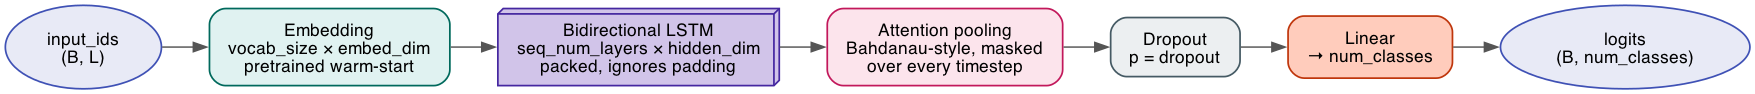
\includegraphics[width=0.9\textwidth]{bilstm_diagram.png}
\caption{BiLSTMClassifier architecture}
\end{figure}

Two omissions are deliberate, not oversights: \texttt{max\_grad\_norm} (gradient-clipping threshold) is
fixed by CLI/config default rather than tuned --- it's a stability safeguard, not an accuracy
lever, so putting it in $\Lambda$ would spend trials on a dimension unlikely to move the metric.
And unlike \texttt{transformer}, there is no \texttt{freeze\_ratio}-equivalent knob: nothing is pretrained
end-to-end here to freeze in the first place, only the embedding matrix, and that is warm-started
rather than frozen.

\section*{Methodology}

Putting the pieces from the previous sections together, this is what a full search actually
does end to end, from an empty candidate pool to a finished submission.

\begin{figure}[htbp]
\centering
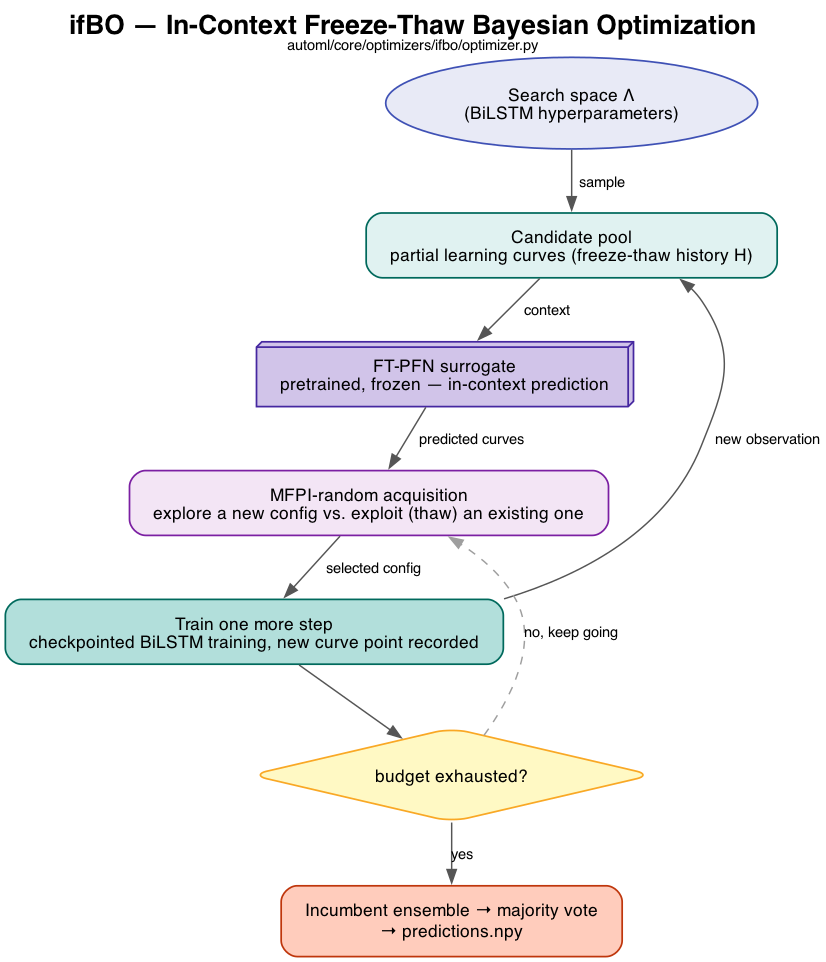
\includegraphics[width=0.9\textwidth]{ifbo_diagram.png}
\caption{The ifBO search loop}
\end{figure}

The search starts with nothing: no configuration has been tried yet, and the candidate pool
is empty. Every iteration opens with a single weighted coin flip that decides whether that
step explores or exploits --- the odds start out heavily favoring exploration, since with an
empty pool there is nothing yet worth exploiting, and gradually shift toward exploitation as
the run progresses and a real pool of partially-trained candidates builds up.

An \textbf{exploration} step is the simple branch: a brand-new configuration is drawn at random
from the search space, dropped straight into the pool, and trained for one step immediately ---
no model, no scoring, no comparison against anything else.

An \textbf{exploitation} step is where the surrogate does its work. Every candidate already in the
pool that hasn't yet been trained to the maximum allowed budget is treated as a contender,
together with one freshly sampled configuration proposed just for this round. All of them are
laid before the surrogate model at once, alongside the complete history of every partial
learning curve observed anywhere in the search so far. The surrogate --- a model trained once,
in advance, and never updated again during the search itself --- reads that history and, for
each contender, predicts how likely it is to cross a target performance level within some
number of additional training steps. Neither the target nor the horizon is fixed: both are
redrawn at random on every single round, so the search never commits to one fixed idea of
``how much better'' or ``how far ahead,'' and instead samples from a broad spread of possible
answers each time. Whichever contender comes out on top is the one trained further. If that
happens to be the freshly proposed configuration, it earns a permanent place in the pool;
otherwise it's discarded and never considered again.

Whichever branch fires, the chosen configuration is then trained for exactly one more
increment, its progress is checkpointed, and the new point on its learning curve is appended
to the shared history the surrogate will read on the next round. This one-step-at-a-time
cycle --- decide, maybe consult the surrogate, train a little further, record the result ---
repeats until the overall budget of decisions runs out.

At the end of the run, rather than keeping only the single best configuration ever seen, the
strongest handful found across the whole search are retrained to completion and combined by
majority vote, and it is that ensemble's predictions that make up the final submission.

\section*{Results}

Budget:

\begin{verbatim}
max_budget: 10
min_budget: 3
n_trials: 20
\end{verbatim}

\subsection*{Baselines}

Three baselines, each isolating a different piece of what makes the flagship method work ---
every one answers a specific ``would doing less still work?'' question rather than just being an
arbitrary point of comparison:

\begin{itemize}
    \item \textbf{Random Search} --- no multi-fidelity behavior at all: every trial
    samples a fresh configuration uniformly from $\Lambda$ and trains it straight through to
    \texttt{max\_budget} epochs before it's ever compared against anything else. It never resumes a
    partially-trained config and never cuts a bad one short. This is the floor every other method
    has to beat to justify its extra machinery, and it also sets an upper bound on wall-clock cost
    per trial, since it always pays for the \emph{full} epoch budget regardless of how a config is
    doing partway through (see the wall-clock comparison below --- this is exactly why its bars are
    tallest everywhere).
    \item \textbf{SMAC (BO+HB)} --- SMAC3's random-forest-surrogate Bayesian
    optimization, paired with a Hyperband intensifier for multi-fidelity scheduling (successive
    halving: only the top fraction of configs at each rung's budget get promoted to the next,
    larger one). This isolates what a \emph{classical, non-neural} multi-fidelity method achieves under
    the same epoch-budget range as ifBO --- the fairest like-for-like comparison against the
    flagship method, since both get to allocate budget adaptively instead of uniformly, but SMAC
    does it with a random-forest-EI surrogate and a handful of \emph{discrete} Hyperband rungs, instead
    of FT-PFN's in-context transformer and \emph{continuous} freeze-thaw (visible directly in the
    fidelity-allocation figure below: SMAC's budget trace is a coarse two-level sawtooth, ifBO's
    is a much finer staircase).
    \item \textbf{ifBO (random selection)} --- runs the \emph{exact same} freeze-thaw pipeline and candidate-pool
    machinery as the flagship method, but with \texttt{ifbo\_use\_random\_selection=True}: FT-PFN's MFPI-random scoring is swapped for a uniform random choice among that round's contenders (pending candidates + one fresh proposal). This is the
    most targeted ablation of the three --- everything about \emph{how much} budget is spent
    incrementally vs.\ upfront is held identical to the flagship run, so any gap between this and
    full ifBO isolates the value of the \emph{surrogate's guidance specifically}, separate from the
    value of freeze-thaw scheduling in general.
\end{itemize}

\subsection*{Testbed Results}



\end{document}